\documentclass{beamer}

\usepackage{pgf,pgfpages}
\usepackage{graphicx}
\usepackage{units}
\usepackage[utf8]{inputenc}

\mode<presentation>
{
  \usetheme{ift}
  \setbeamercovered{transparent}
  \setbeamertemplate{items}[square]
}

\usefonttheme[onlymath]{serif}
\setbeamerfont{frametitle}{size=\LARGE,series=\bfseries}

\definecolor{uibred}{RGB}{170, 0, 0}
\definecolor{uibblue}{RGB}{0, 84, 115}
\definecolor{uibgreen}{RGB}{119, 175, 0}
%\definecolor{uibgreen}{RGB}{50, 105, 0}
\definecolor{uiborange}{RGB}{217, 89, 0}


\beamertemplatenavigationsymbolsempty


%====================================================
%-------------Macro definitions go here--------------
%====================================================

%
% Differentials
%
\newcommand{\tdiff}[2]{\ensuremath{\frac{\mathrm{d}#2}}{\mathrm{d}{#1}}}
\newcommand{\tdifforder}[3]{\ensuremath{\frac{\mathrm{d}^{#2}#3}{\mathrm{d}{#1}^{#2}}}}
\newcommand{\pdiff}[2]{\ensuremath{\frac{\partial#2 }{\partial#1}}}
\newcommand{\pdifforder}[3]{\ensuremath{\frac{\partial^{#2}#3}{\partial{#1}^{#2}}}}

% bracket
\newcommand{\bra}[1]{\ensuremath{\left<#1\right|}}
\newcommand{\ket}[1]{\ensuremath{\left|#1\right>}}
\newcommand{\bracket}[2]{\ensuremath{ \left\langle #1 | #2 \right\rangle}}
\newcommand{\matelem}[3]{\ensuremath{ \left\langle #1 | #2 | #3 \right\rangle}}
\newcommand{\matr}[1]{\ensuremath{\mathbf{#1}}}
\newcommand{\vect}[1]{\ensuremath{\mathbf{#1}}}
\newcommand{\expectationvalue}[1]{\ensuremath{\left\langle #1 \right\rangle}}

\renewcommand{\imath}{\ensuremath{\mathrm{i}}}

%
% Linear algebra
%
\renewcommand{\vec}[1]{\ensuremath{\mathbf{#1}}}
\newcommand{\mat}[1]{\ensuremath{\mathbf{#1}}}
\newcommand{\tildemat}[1]{\ensuremath{\widetilde{\mat{#1}}}}

% Numerical analysis
\newcommand{\bigo}{\ensuremath{\mathcal{O}}}
\renewcommand{\Re}{\ensuremath{\mathrm{Re}}}
\renewcommand{\Im}{\ensuremath{\mathrm{Im}}}
\newcommand{\mathcol}[2]{{\color{#1}#2}}
\newcommand{\red}[1]{\mathcol{uibred}{#1}}
\newcommand{\blue}[1]{\mathcol{uibblue}{#1}}
\newcommand{\green}[1]{\mathcol{uibgreen}{#1}}
\newcommand{\orange}[1]{\mathcol{uiborange}{#1}}
%
% Misc macros
%
\newcommand{\eref}[1]{~(\ref{#1})}
\renewcommand{\equiv}[0]{\ensuremath{:=}}
\newcommand{\etal}{\textit{et al. }}
\newcommand{\paperheader}[2]{\noindent\textbf{Paper #1}: \textit{#2}\\}
\newcommand{\paperitem}[3]{\noindent\textbf{Paper #1}: \textit{#2}\vspace{1em}\\\noindent #3\vspace{2em}}
\newcommand{\tfinal}{\ensuremath{T_{\text{f}}}}
\newcommand{\papernum}[1]{\textbf{#1}}
%\newcommand{\note}[1]{\colorbox{yellow}{#1}}
\newcommand{\paperref}[1]{Paper~\textbf{#1}}

%
% Code
%
\newcommand{\inlinename}[1]{\lstinline[basicstyle=\ttfamily,language=bash]{#1}}




%\includeonlyframes{current}


\defbeamertemplate{enumerate item}{mycircle}
{
  %\usebeamerfont*{item projected}%
  %\usebeamercolor[bg]{item projected}%
  \begin{pgfpicture}{0ex}{0ex}{1.5ex}{0ex}
	%\pgfcircle[fill]{\pgfpoint{0pt}{.75ex}}{1.25ex}
    \pgfbox[center,base]{\color{uibblue}\insertenumlabel.}
  \end{pgfpicture}%
}
[action]
{\setbeamerfont{item projected}{size=\scriptsize}}
\setbeamertemplate{enumerate item}[mycircle]




\title{PyProp - A Python Framework for Propagating the Time Dependent Schrödinger Equation}
\author{Tore Birkeland}
\institute{
Department of Mathematics, University of Bergen
}
\date{December 18, 2009}

\begin{document}


\setbeamertemplate{background}
 {
\includegraphics[width=\paperwidth,height=\paperheight]{frontpage_bg}}
\setbeamertemplate{footline}[default]

\begin{frame}
  \titlepage
  \vspace{5cm}
\end{frame}

%
% Set the background for the rest of the slides.
% Insert infoline at the end
%
\setbeamertemplate{background}
 {
\includegraphics[width=\paperwidth,height=\paperheight]{slide_bg}}
\setbeamertemplate{footline}[ifttheme]

%--------------------------------------------------------------------
%                          Introduction
%--------------------------------------------------------------------

\section{Introduction}

%\begin{frame}
%	\frametitle{The Title}
%	\begin{itemize}
%		\item PyProp 
%		\item Python 
%		\item Framework 
%		\item Propagating 
%		\item Time Dependent Schrödinger Equation 
%	\end{itemize}
%	
%\end{frame}


%--------------------------------------------------------------------
%                          Outline
%--------------------------------------------------------------------

\subsection{Motivation}

\begin{frame}
	\frametitle{Underlying Goal}
	
	\begin{center}
		\Large
		Study the behaviour of atoms and molecules
	\end{center}

\end{frame}



%\begin{frame}
%	\frametitle{Why?}
%
%	\begin{columns}
%		\column{0.4\textwidth}
%		\begin{center}
%			\parbox[c][0.8\textheight]{0.9\textwidth}
%			{
%				\includegraphics<1>[width=0.8\textwidth]{figurer/images/molecule.png}
%				\includegraphics<2>[width=\textwidth]{figurer/images/chip.jpg}
%				\includegraphics<3>[width=\textwidth]{figurer/images/star.jpg}
%			}
%		\end{center}
%		\column{0.6\textwidth}
%			\begin{itemize}
%				\item<1-> Understand the foundations of chemistry, 
%				\item<2-> Develop faster computers
%				\item<3-> Understand the fundamental processes in stars
%			\end{itemize}
%	\end{columns}
%
%\end{frame}
%


\begin{frame}
	\frametitle{Length Scale}
% images
% ant - http://commons.wikimedia.org/wiki/File:Meat_eater_ant_feeding_on_honey02.jpg
% hair - http://commons.wikimedia.org/wiki/File:Human_Hair_40x.JPG
% droplet - http://commons.wikimedia.org/wiki/File:Rainbow_droplet.jpg
% cell - http://commons.wikimedia.org/wiki/File:SEM_blood_cells.jpg
% hiv - http://en.wikipedia.org/wiki/File:HIV-budding-Color.jpg

	\begin{columns}
		\column{0.4\textwidth}
			\parbox[c][0.8\textheight]{0.9\textwidth}
			{
				\includegraphics<1>[width=\textwidth]{figurer/images/scale_0}
				\includegraphics<2>[width=\textwidth]{figurer/images/scale_2}
				\includegraphics<3>[width=\textwidth]{figurer/images/scale_4}
				\includegraphics<4>[width=\textwidth]{figurer/images/scale_6}
				\includegraphics<5>[width=\textwidth]{figurer/images/scale_8}
				\includegraphics<6>[width=\textwidth]{figurer/images/scale_10}
			}
		
		
		\column{0.6\textwidth}
			\begin{tabular}{l l l}
				\onslide<1->{$10^{0}\unit{m}$  } &  & \onslide<1->{Humans} \\
				\onslide<2->{$10^{-2}\unit{m}$ } &  & \onslide<2->{Golf balls} \\
				\onslide<3->{$10^{-4}\unit{m}$ } &  & \onslide<3->{Width of human hair} \\
				\onslide<4->{$10^{-6}\unit{m}$ } &  & \onslide<4->{Cells} \\
				\onslide<5->{$10^{-8}\unit{m}$ } &  & \onslide<5->{Vira} \\
				\onslide<6->{$10^{-10}\unit{m}$} &  & \onslide<6->{Atoms} \\
			\end{tabular}
	\end{columns}
\end{frame}


\begin{frame}
	\frametitle{How?}

	\parbox[c][4.5cm]{\textwidth}
	{
		\begin{center}
			\includegraphics<1-2>[width=6cm]{figurer/wavelength_atom}
			\includegraphics<3>[width=6cm]{figurer/experiment_1}
			\includegraphics<4->[width=6cm]{figurer/experiment_2}
		\end{center}
	}

	\begin{itemize}
		\item<1-> Atoms are smaller than the wavelength of light
		\item<2-> Any observation leads to a modification of the system
		\item<3-> It is not possible to directly observe what is going on
		\item<5-> Need theoretical models and calculations to match experiments
	\end{itemize}
	
\end{frame}

\begin{frame}
	\frametitle{Numerical Experiment}

	\textit{Simulation of an experimental setup on a computer}

	\begin{enumerate}
		\item<2-> An atomic/molecular system is in an initial state
		\item<3-> The system interacts with an external force
			\begin{itemize}
				\item Interaction with radiation (laser)
				\item Collision with another atom/ion/molecule
			\end{itemize}
		\item<4-> The final state of the system is analyzed to compare with experiments
	\end{enumerate}	
	\vspace{0.5cm}

	\onslide<5->
	{
		The goal of this thesis is to perform steps 1 and 2 and simplify step 3 for a wide range of problems
	}
\end{frame}


\subsection{Outline}

\begin{frame} % frame
	\frametitle{Outline}
	\begin{itemize}
		\item Overview of the thesis
		\item Introduction to Quantum Mechanics
		\item Solving the Time Dependent Schrödinger Equation on a computer
		\item How PyProp is a flexible solver 
		\item Applying PyProp to laser ionization of Helium
	\end{itemize}
\end{frame}


\section{Overview}

\begin{frame}
	\frametitle{Thesis Overview}

	Development and application of PyProp
	\begin{itemize}
		\item Computer Science - Software design and implementation
		\item Mathematics - Numerical methods
		\item Physics - Applications
	\end{itemize}
\end{frame}



\begin{frame}
	\frametitle{What is PyProp?}

	\textit{Framework for solving the Time Dependent Schrödinger Equation}

	\begin{itemize}
		\item<2-> Goals
			\begin{itemize}
				\item Flexibility
				\item Performance
			\end{itemize}
		\item<3-> Research tool, not QM@Home
			\begin{itemize}
				\item Common tasks automated
				\item Difficult tasks possible
			\end{itemize}
		\item<4-> Free Software (GPL) http://pyprop.googlecode.com
	\end{itemize}
\end{frame}




\begin{frame}
	\frametitle{Scientific Results}
	\tiny

	\vspace{0.25cm}
	\begin{enumerate}
		\item
			{\color<2->{gray}
			\underline{T. Birkeland}, M. Førre, J. P. Hansen and S. Selstø, \textit{Dynamics of H$_{2p}$ ionization in ultrashort strong laser pulses}, J. Phys. B At. Mol. Opt. Phys, \textbf{37} 4205-4219 (2004)
			}
		\item 
			{\color<2->{uibgreen}
			\underline{T. Birkeland} and T. Sørevik
			\textit{Parallel Redistribution of Multidimensional Data}
			Proceedings ParCo 2007 Conference
			NIC Series Volume \textbf{38}, (2007)
			}
		\item
			{\color<2->{uibgreen}
			V. Popsueva, R. Nepstad, \underline{T. Birkeland}, M. Førre, J. P. Hansen, E. Lindroth and E. Waltersson,
			\textit{Structure of lateral two-electron quantum dot molecules in electromagnetic fields}
			{Physical Review} B, \textbf{76}, 035303 (2007)
			}
		\item
			{\color<2->{uibgreen}
			L. Sælen, I. Sundvor, \underline{T. Birkeland}, S. Selstø, and M. Førre, 
			\textit{Classical and quantum-mechanical investigation of the role of nondipole effects on the binding of a stripped HD$^{2+}$ molecule}
			{Physical Review} A, \textbf{76}, 013415 (2007)
			}
		\item
			{\color<2->{uibgreen}
			T. Sørevik, \underline{T. Birkeland} and G. Okša, 
			\textit{Numerical solution of the 3D time dependent Schrödinger equation in
		spherical coordinates: Spectral basis and effects of split-operator
		technique}
			{Journal of Computational and Applied Mathematics}, \textbf{225}, 56-67 (2007) 
			}
		\item
			{\color<2->{uibgreen}
			C. R. Calvert, \underline{T. Birkeland}, R. B. King, I. D. Williams and J. F. McCann, 
			\textit{Quantum chessboards in the deuterium molecular ion}
			{J. Phys. B: At. Mol. Opt. Phys.}, \textbf{41}, 205504 (2008)
			}
		\item
			{\color<2->{uibgreen}\color<3->{uibred} 
			\underline{T. Birkeland} and T. Sørevik, 
			\textit{Parallel Pseudo-spectral Methods for the Time Dependent Schrödinger Equation}
			{Parallel Computing: Numerics, Applications, and Trends}
			R. Trobec, M Vajteršic and P. Zinterhof (ed.) 261-279 (2009) 
			}
		\item
			{\color<2->{gray}
			C. R. Calvert, R. B. King, \underline{T. Birkeland}. J. D.  Alexander, J. B. Greenwood, W. A. Bryan, W. R. Newell, D. S. Murphy, J. F. McCann and I. D. Williams, 
			\textit{Pathways to state-selective control of vibrational wavepackets in the deuterium molecular ion} Journal of Modern Optics, \textbf{56} 1060-1069 (2009) 
			}
		\item
			{\color<2->{gray}
			\underline{T. Birkeland} and R. Strand, 
			\textit{How to Understand Nano Images},
			Techne: Research in Philosophy and Technology, in print (2009)
			}
		\item
			{\color<2->{gray}
			R. Strand and \underline{T. Birkeland}, 
			\textit{The Science and Politics of Nano Images} Nano meets Macro: Social Perspectives on Nanoscale Sciences and Technologies, (2009)
			}
		\item
			{\color<2->{gray}
			L. Sælen, \underline{T. Birkeland}, N. Sisourat, A. Dubois and J. P. Hansen, 
			\textit{Full 3D ab initio studies of interference effects in high-energy ion-molecule collisions} Proceedings of ICPEAC XXVI, in print (2009)
			}
		\item
			{\color<2->{uibgreen}
			L. Sælen, \underline{T. Birkeland}, N. Sisourat, A. Dubois and J. P. Hansen, 
			\textit{Non perturbative treatment of single ionization of $H_2$ by fast, highly charged ion impact},
			submitted for publication (2009)
			}
		\item
			{\color<2->{uibgreen}\color<3->{uibred}
			\underline{T. Birkeland}, R. Nepstad and M. Førre,  
			\textit{Multiphoton Double Ionization in Helium Driven by Intense XUV Attosecond Pulses},
			to be submitted 
			}
	\end{enumerate}
\end{frame}




\subsection{Introduction to Quantum Mechancis}

\begin{frame}
	\frametitle{Classical Mechanics}

	\begin{columns}
		\column{0.25\textwidth}
%			\includegraphics<1>[width=\textwidth]{figurer/classical_particle_1}
			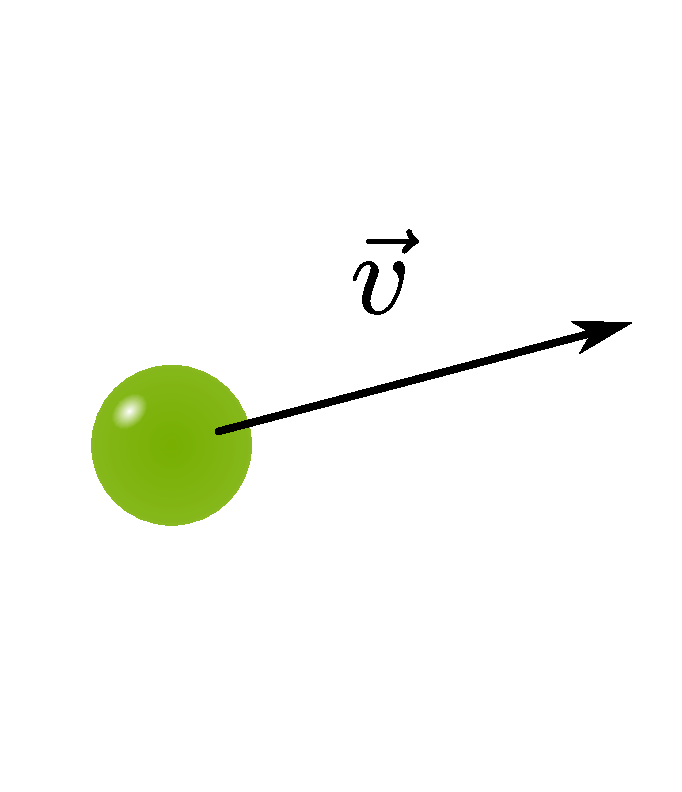
\includegraphics[width=\textwidth]{figurer/classical_particle_2}

		\column{0.75\textwidth}
			A classical particle has a well defined position and velocity.
			\vspace{0.5cm}


			The change of velocity is described by Newton's Law
			\begin{equation*}
				\vect{F} = m \vect{a}
			\end{equation*}
	\end{columns}
\end{frame}

%\begin{frame}
%	\frametitle{Calculations in Classical Mechanics}
%
%	\begin{eqnarray*}
%		\tdiff{t}{x} &=& v \\
%		\tdiff{t}{v} &=& F / m
%	\end{eqnarray*}
%\end{frame}


\begin{frame}
	\frametitle{Quantum Mechanics}

	\begin{columns}
		\column{0.4\textwidth}
			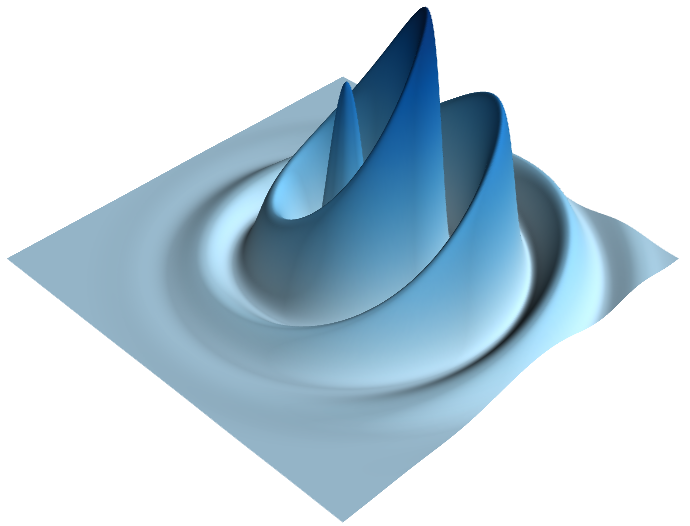
\includegraphics[width=\textwidth]{figurer/quantum_particle}

		\column{0.6\textwidth}
			Heisenberg uncertainty principle: a particle can not have well defined position and velocity
			\begin{itemize}
				\item<2-> There is a probability for finding a particle in a given position
				\item<3-> Must therefore consider all possible positions at the same time
			\end{itemize}
	\end{columns}
\end{frame}


\begin{frame}
	\frametitle{Mathematical Formulation}

	\onslide<1->{
		Position and velocity is replaced by a \emph{wavefunction}
		\begin{equation*}
			\psi(\vect{x},t)	
		\end{equation*}
		$|\psi(\vect{x},t)|^2$ is the probability density of finding the particle in $\vect{x}$\\
	}
	
	\vspace{1cm}
	\onslide<2->{
	Time evolution of $\psi(\vect{x},t)$ is described by the Time Dependent Schrödinger Equation (TDSE).
		\begin{equation*}
			\imath \pdiff{t}{}\psi(\vect{x},t) = \widehat{H} \psi(\vect{x},t)
		\end{equation*}
	}
\end{frame}

\begin{frame}
	\frametitle{Hamiltonian}

	The Hamiltonian describes the energies in the system
	\parbox[c][2cm]{\textwidth} 
	{
		\begin{equation*}
			\widehat{H} = {\color<2>{uibred} -\frac{1}{2m} \nabla^2} + {\color<3->{uibred} V(\vect{\vect{x}}, t)}
		\end{equation*}

	}
	\begin{itemize}
		\item<2-> The differentiation operator represents kinetic energy
		\item<3-> $V(\vect{x})$ is the potential energy.
		\item<4-> Systems are characterized by different potentials
	\end{itemize}

\end{frame}


\begin{frame}
	\frametitle{Adding Particles}

	\begin{itemize}
		\item Adding a particle is equivalent to adding degrees of freedom
	\end{itemize}
	\onslide<2->
	{
	\begin{equation*}
		\imath \pdiff{t}{}\psi(\vect{x}_1, \vect{x}_2, t) = \left(H_1(\vect{x}_1) + H_2(\vect{x}_2) + H_{1,2}(\vect{x}_1, \vect{x}_2) \right) \psi(\vect{x}_1, \vect{x}_2, t) 
	\end{equation*}
	}
	\begin{itemize}
		\item<3-> The time for solving a system increases exponentially with the number of particles
		\begin{itemize}
			\item<4-> 1 particle: 1 sec
			\item<5-> 2 particles: 17 min
			\item<6-> 3 particles: 277 hours
			\item<7-> 7 particles: age of the universe
		\end{itemize}
		\item<8-> The ``exponential wall'' of quantum mechanics
	\end{itemize}
	
\end{frame}


%\begin{frame}
%	\frametitle{Adding degrees of freedom}
%
%	\begin{itemize}
%		\item with one degree of freedom, there is only one axis where the particle can move.
%		\item Adding a degree of freedom (2D), the particle can be found anywhere on a plane
%	\end{itemize}
%	\begin{equation*}
%		\psi(x,y)
%	\end{equation*}
%	\begin{itemize}
%		\item When discretizing each degree of freedom with $m$ independent variables, the size of the wavefunction grows exponentially with the number of degrees of freedom
%	\end{itemize}
%
%\end{frame}

\section{Computational Quantum Mechanics}

\begin{frame}
	\frametitle{Computational Quantum Mechanics}

	Returning to the TDSE
	\begin{equation*}
		\imath \pdiff{t}{}\psi(\vect{x},t) = \widehat{H} \psi(\vect{x},t)
	\end{equation*}

	\onslide<2->
	{
		Problem: if we know the $\psi(\vect{x}, t)$, find $\psi(\vect{x}, t+h)$.
	}
	\vspace{0.25cm}


	\begin{itemize}
		\item<3-> Can only be solved by hand for the simplest systems
		\item<4-> Computers does not work on continuous problems, the TDSE must therefore be \emph{discretized} in space and time. 
	\end{itemize}

\end{frame}


\subsection{Space Discretization}

\begin{frame}
	\frametitle{Choice of coordinate system}

	Must choose a coordinate system in which to represent the multi-dimensional wavefunction.
	\vspace{0.5cm}

	\begin{columns}
		\column{0.3\textwidth}
			\includegraphics<1-2>[width=\textwidth]{figurer/cartesian_with_grid.png}
			\includegraphics<3>[width=\textwidth]{figurer/spherical_with_grid.png}
			\includegraphics<4->[width=\textwidth]{figurer/cylindrical_with_grid.png}
		
		\column{0.6\textwidth}
			\begin{itemize}
				\item<2-> Cartesian coordinates, $\vect{x} = (x,y,z)$
				\item<3-> Spherical coordinates, $\vect{x} = (r, \theta, \phi)$
				\item<4-> Cylindrical coordinates, $\vect{x} = (r, \rho, \phi)$
				\item<5-> Each rank may be discretized independently
				\item<6-> Optimal choice is system dependent
			\end{itemize} 
	\end{columns}

\end{frame}




\begin{frame}
	\frametitle{Discretization}
	
	\begin{itemize}
		\item<1-> Approximating the continuous problem with a finite number of states.
		\item<2-> Sum of continuous basis functions 
	\end{itemize}
	\onslide<2->
	{
	\begin{equation*}
		\psi(x,t) \approx \sum_{i=0}^m c_i(t) B_i(x)
	\end{equation*}
	}
	\begin{itemize}
		\item<3-> Perform calculations on $\vect{c}(t) = \{ c_i(t) \}$
		\item<4-> Which basis functions should we use?
		\begin{itemize}
			\item Fourier functions?
			\item Orthogonal polynomials?
			\item B-Splines?
		\end{itemize}
		\item<5-> Optimal choice is system dependent
	\end{itemize}
\end{frame}


\subsection{Time Discretization}

\begin{frame}
	\frametitle{Propagation}

	Given a discretization scheme, we can turn the TDSE from 
	\begin{equation*}
		\imath \pdiff{t}{}\psi(\vect{x},t) = \widehat{H} \psi(\vect{x},t) 
		\hspace{0.5cm}\rightarrow\hspace{0.5cm}
		\imath \matr{S} \pdiff{t}{}\vect{c}(t) = \matr{H} \vect{c}(t)
	\end{equation*}

	\begin{itemize}
		\item<2-> Propagation: from $\vect{c}(t)$, find $\vect{c}(t+h)$
		\item<3-> Choice of propagation scheme
			\begin{itemize}
				\item Cayley Propagator
				\item Split-Step Propagator
				\item Krylov Propagator
			\end{itemize}
		\item<4-> Can be done independently from space discretization
%			\begin{itemize}
%				\item However, some discretization schemes favors certain propagation schemes.
%			\end{itemize}
		\item<5-> Optimal propagation scheme is system dependent
	\end{itemize}
	
\end{frame}


\subsection{Making a Flexible Solver}

\begin{frame}
	\frametitle{Solving the TDSE - Summary}

	\begin{itemize}
		\item System dependent choices
			\begin{itemize}
				\item coordinate system
				\item discretization scheme
				\item propagator
			\end{itemize}
		\item<2-> Making the right choice is difficult
		\item<3-> The wrong choice can lead to hard-to-solve systems
		\item<4-> A flexible solver should allow experimentation with different methods
	\end{itemize}

\end{frame}


\section{PyProp}

\begin{frame}
	\frametitle{PyProp Framework Design}

	\begin{columns}
		\column{5cm}
			\begin{itemize}
				\item<2->{\color{uibblue} Core Routines}
				\item<3->{\color{uibred} Independent Modules}
				\item<4->{\color{uibgreen} User Code}
			\end{itemize}

		\column{7cm}
			\includegraphics<2>{figurer/framework-1}
			\includegraphics<3>{figurer/framework-2}
			\includegraphics<4>{figurer/framework}
	\end{columns}

\end{frame}

\begin{frame}
	\frametitle{Flexibility}

	\begin{itemize}
		\item<1-> Choose dimensionality and discretization
			\begin{itemize}
				\item Several discretization schemes built in
				\item Can calculate inner products, operator-wavefunction multiplications, load/save wavefunctions
			\end{itemize}
		\item<2-> Supply potentials
			\begin{itemize}
				\item PyProp takes care of a lot of repetetive code
			\end{itemize}
		\item<3-> Choose propagator
			\begin{itemize}
				\item Several propagators built in
			\end{itemize}
		\item<4-> Perform analysis and data exploration
			\begin{itemize}
				\item High level code is written in Python
				\item All the propagation tools can be used interactively
			\end{itemize}
	\end{itemize}
\end{frame}

\begin{frame}
	\frametitle{Performance}

	\begin{itemize}
		\item<1-> Computational kernels are optimized
			\begin{itemize}
				\item Using high performance libraries where possible
				\item Written in C++/Fortran 
			\end{itemize}
		\item<2-> Practical calculations can have wavefunctions with $\unit[1]{B}$ elements.
		\item<3-> Automatic parallelization of one or more ranks
			\begin{itemize}
				\item Supports redistribution
				\item Parallel matrix-vector operations
			\end{itemize}
	\end{itemize}
	
\end{frame}

\subsection{Applications}

\begin{frame}
	\frametitle{Current Applications}
	
	\textbf{Numerics:}
	\begin{itemize}
		\item Generalized reduced wavefunctions (Lundeland and Kozlov)
		\item {\color<2->{uibgreen} Multidimensional Redistribution (ParCo 2007 p443 (2008))}
		\item {\color<2->{uibgreen} Trans. Chebyshev Grids (J. Comp. Appl. Math. 225 p56 (2009))}
	\end{itemize}
	
	\textbf{Physics:}
	\begin{itemize}
		\item {\color<2->{uibgreen} Two Electron Quantum Dots (Phys. Rev. B 76, 035303 (2007))}
		\item {\color<2->{uibgreen} Laser-bound Molecules (Phys. Rev. A 76, 013415 (2007))}
		\item {\color<2->{uibgreen} Vibrational Molecular Wavepackets (J. Phys. B 41 205504 (2008))}
		\item Laser Ionization of SAE Argon (Nepstad et.al. (2009))
		\item {\color<2->{uibgreen} Ion-Molecule Collsion (Submitted)}
		\item {\color<2>{uibgreen}\color<3->{uibred}Laser Ionization of Two-Electron Helium (In preparation)}
		\item Laser Ionization of $H_2$ (work in progress)
		\item Born-Oppenheimer effects in $H_2^+$ (work in progress)
	\end{itemize}

\end{frame}

\subsection{Laser Ionization of Helium}

\begin{frame}
	\frametitle{Example: Laser Ionization of Helium}

	\begin{center}
		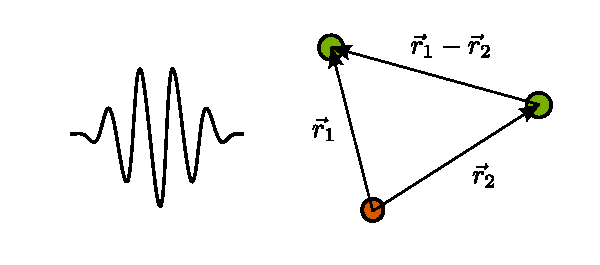
\includegraphics[height=3cm]{figurer/helium}
	\end{center}
	\vspace{-1cm}

	\begin{itemize}
		\item Two electron system
	\end{itemize}
	\vspace{-1cm}

	\begin{eqnarray*}
		\widehat{H}_0(\vect{r}_i) &=& -\frac{1}{2} \nabla^2 - \frac{2}{r_i}  + A_z(t) \left( \pdiff{z_i}{} - \frac{\cos \theta_i}{r_i} \right)\\
		\onslide<2->{ \widehat{H}(\vect{r}_1,\vect{r}_2)   }
		& \onslide<2->{=}& 
		\onslide<2->{\widehat{H}_0(\vect{r}_1) + \widehat{H}_0(\vect{r}_2) + \frac{1}{|\vect{r}_1 - \vect{r}_2|} }
	\end{eqnarray*}
	\vspace{-0.5cm}

	\begin{itemize}
		\item<3-> Near spherical symmetry around the nucleus
	\end{itemize}
\end{frame}

\begin{frame}
	\frametitle{Helium in PyProp}

	\begin{itemize}
		\item<1-> Three computational ranks
			\begin{enumerate}
				\item $\mathcal{Y}_{l_1,l_2}^{L,M}(\Omega_1, \Omega_2)$ - Combination of all angles
				\item $r_1$ - distance from nucleus to first electron 
				\item $r_2$ - distance from nucleus to second electron 
			\end{enumerate}
		\item<2-> Discretizing $r_1$ and $r_2$ with B-Splines 
		\item<3-> Total wavefunction has $\approx \unit[10]{M}$ elements
			\begin{itemize}
				\item Total memory requirement is $\approx \unit[100]{GB}$
				\item Must be run in parallel 
			\end{itemize}
		\item<4-> Propagation with the Cayley Propagator
		\item<5-> A calculation typically takes $\unit[24]{h}$ on $\unit[111]{CPUs}$
	\end{itemize}
\end{frame}


\begin{frame}
	\frametitle{Helium - Analysis}
	
	\begin{itemize}
		\item<2-> Determine physical quantities
			\begin{itemize}
				\item Ionization probability
				\item Energy distribution
			\end{itemize}
		\item<3-> Remove bound states
			\begin{itemize}
				\item Use integrated eigenvalue solver 
			\end{itemize}
		\item<4-> Project wavefunction on single electron states
			\begin{itemize}
				\item Use the same discretization and propagation schemes for single electron problems
			\end{itemize}
	\end{itemize}
\end{frame}


\begin{frame}
	\frametitle{Helium - Movie}

	\begin{center}
		Animation of an ionization event
	\end{center}
\end{frame}


\begin{frame}
	\frametitle{Helium - Ionzation Probability}

	\begin{center}
		Ionization probability as a function of field strength
		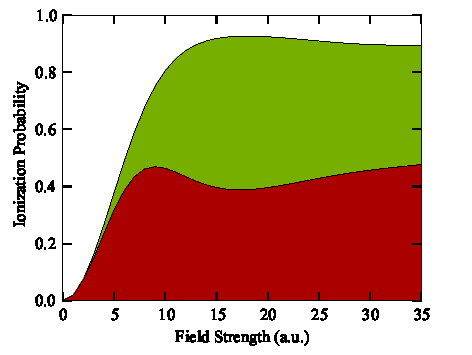
\includegraphics[width=7cm]{figurer/1s1s_ionization_probability.pdf}
	\end{center}
	\vspace{-0.8cm}
	\begin{itemize}
		\item Ionization probability does not go to one
		\item Each point on the graph is from one ionization event
			\begin{itemize}
				\item Total of 30000 CPU hours
			\end{itemize}
	\end{itemize}
\end{frame}


\section{Outlook and summary}

\begin{frame}
	\frametitle{Summary}

	\begin{itemize}
		\item<1-> Created a software framework for atomic physics
			\begin{itemize}
				\item<2-> Scalable - can perform massive calculations on large 2 electron systems
				\item<3-> Flexible - can combine many different discretizations and propagators to solve quite diverse problems
			\end{itemize}
		
		\item<4-> Solved a variety of problems using PyProp
	\end{itemize}
\end{frame}


\begin{frame}
	\frametitle{Future plans}
	
	\begin{itemize}
		\item<1-> Ease transition for new users
			\begin{itemize}
				\item<2-> Documentation
				\item<3-> Simplify installation procedure
				\item<4-> Better error handling
			\end{itemize}
		\item<5-> Compare methods
		\item<6-> Simplify implementation of new methods
	\end{itemize}
\end{frame}



\begin{frame}
	\frametitle{Image Sources}

	\textbf{Wikimedia Commons}
	\begin{itemize}
		\item Vitruvian man - File:Vitruvian.jpg
		\item Hair - File:Human\_Hair\_40x.JPG
		\item Cell - File:SEM\_blood\_cells.jpg
		\item HIV - File:HIV-budding-Color.jpg
		\item Atom - File:Stylised\_Lithium\_Atom.svg
	\end{itemize}

	\textbf{Raymond Nepstad}
	\begin{itemize}
		\item Wavefunction
		\item Helium animation
	\end{itemize}
	
\end{frame}
\end{document}

